\section{Ping pong}\label{sec:pingpong}

\begin{lemma}[Ping pong]\label{lem:pingpong}
Let $a$ and $b$ act on a set $X$, and let $X_a, X_b \subseteq X$ be disjoint and
nonempty. Suppose $a^n(X_b) \subseteq X_a$ and $b^n(X_a) \subseteq X_b$ for
every $n \neq 0$. Then $\langle a, b \rangle$ is free on $a$ and $b$.
\end{lemma}

\begin{proof}
A nontrivial reduced word in $a$ and $b$ is conjugate to one of the form
$w = a^{n_k} b^{m_{k-1}} \cdots b^{m_1} a^{n_1}$ with every exponent nonzero.
Each letter moves $X_b$ into $X_a$ or $X_a$ into $X_b$ in turn, so
$w(X_b) \subseteq X_a$. Since $X_a \cap X_b = \emptyset$, $w$ is not the
identity.
\end{proof}

\begin{theorem}[Sanov]\label{thm:sanov}
The matrices
\[
  A = \begin{pmatrix} 1 & 2 \\ 0 & 1 \end{pmatrix}, \qquad
  B = \begin{pmatrix} 1 & 0 \\ 2 & 1 \end{pmatrix}
\]
generate a free subgroup of $\SL_2(\Z)$ of rank two.
\end{theorem}

\begin{proof}
Let $\SL_2(\Z)$ act on $\R \cup \{\infty\}$ by M\"obius transformations, and set
$X_A = \{x : |x| > 1\}$ and $X_B = \{x : |x| < 1\}$. If $|x| < 1$ then
$|A^n x| = |x + 2n| > 2|n| - 1 \geq 1$, so $A^n(X_B) \subseteq X_A$. If
$|x| > 1$ then $B^n x = x/(2nx + 1)$ and $|1/B^n x| = |2n + 1/x| > 1$, so
$B^n(X_A) \subseteq X_B$. Apply Lemma~\ref{lem:pingpong}.
\end{proof}

\begin{figure}[ht]
\centering
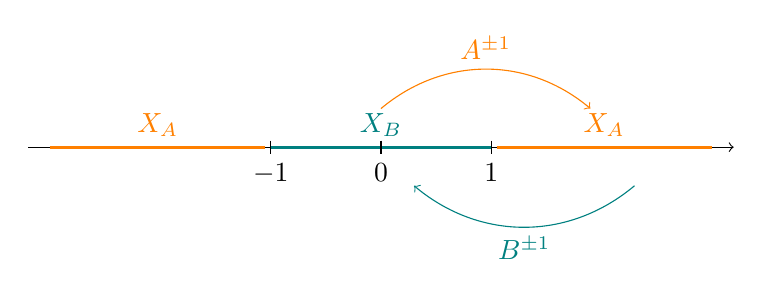
\begin{tikzpicture}[scale=1.4]
  \draw[->] (-3.2,0) -- (3.2,0);
  \draw[very thick, teal] (-1,0) -- (1,0) node[midway, above] {$X_B$};
  \draw[very thick, orange] (-3,0) -- (-1.05,0) node[midway, above] {$X_A$};
  \draw[very thick, orange] (1.05,0) -- (3,0) node[midway, above] {$X_A$};
  \foreach \x in {-1,0,1} \draw (\x,0.06) -- (\x,-0.06) node[below] {$\x$};
  \draw[->, orange] (0,0.35) to[bend left=40] node[above] {$A^{\pm1}$} (1.9,0.35);
  \draw[->, teal] (2.3,-0.35) to[bend left=40] node[below] {$B^{\pm1}$} (0.3,-0.35);
\end{tikzpicture}
\caption{The ping-pong sets for Theorem~\ref{thm:sanov}.}\label{fig:pingpong}
\end{figure}
